%-------------------------- Classe --------------------------%

%% Ce document a été produit par Antoine FAYOLLE à l'attention des étudiants de l'université de Tours

\documentclass[11pt]{article}
\setlength{\textwidth}{400pt}


%-------------------------- Packages --------------------------%

\usepackage[utf8]{inputenc} %Permet d'utiliser tous les caractères utf8
\usepackage[T1]{fontenc} %L’encodage T1 (également appelé Cork encoding) est conçu pour supporter les langues européennes et offre une meilleure gestion des caractères accentués
\usepackage[french,english]{babel} % Permet de traduire automatiquement certaines commandes (telle que le titre de la table des matières), la langue peut être changée grâce à la commande : \selectlanguage{language}
\usepackage{amsmath} %check : http://www.ams.org/arc/tex/amsmath/amsldoc.pdf
\usepackage{bm} % Pour mettre en gras tous les symboles en mode math : \bm
\usepackage{fancyhdr} % Pour la mise en page
%\usepackage{pdftricks2}
\usepackage{amsfonts} % Pour plus de polices mathématiques avec \mathbb{} et \mathcal{}
\usepackage{empheq} %Pour avoir des systèmes d'équations avec une accolade et une numérotation du type (3a),(3b) : \begin{subequations} \begin{empheq}[left=\empheqlbrace]{align} ... \end{empheq} \end{subequations}
\usepackage{graphicx} % Pour les figures, check : https://texdoc.org/serve/graphicx.pdf/0 
\usepackage{wrapfig} % Pour insérer des images dans le texte
\usepackage{wallpaper} %check : https://texdoc.org/serve/wallpaper/0
\usepackage[pdftex, hidelinks]{hyperref} % Permet d'avoir des liens et hyper liens dans le document pdf, avec ces arguments optionnels ils sont invisibles, check : https://texdoc.org/serve/hyperref/0 
\usepackage{physics} %for matrixes, \dd, \dv, \bra, \ket and \braket, check : https://mirrors.ibiblio.org/CTAN/macros/latex/contrib/physics/physics.pdf
\usepackage[a4paper, total={450pt, 700pt}, voffset=30pt]{geometry} %Pour la mise en page, check : https://texdoc.org/serve/geometry.pdf/0
\usepackage[acronym,nonumberlist,nomain]{glossaries-extra} %Pour avoir un glossaire d'acronymes
\setabbreviationstyle[acronym]{long-short}
\makeglossaries
\usepackage{enumitem} %Pour avoir des listes sans puce
\usepackage{listings} %Pour insérer du code dans le document
\definecolor{light-gray}{gray}{0.95} %Pour avoir un gris clair derrière le code
\lstset{ basicstyle=\footnotesize, escapechar=\£, showstringspaces=false, backgroundcolor=\color{light-gray}} % Ajout d'une commande pour utiliser des macros dans les environnements verbatim, définit la police et la couleur d'arrière-plan dans les environnements lstlisting
\usepackage{perpage} %Pour réinitialiser automatiquement à chaque nouvelle page la numérotation des notes de bas de page
\MakePerPage{footnote}
\renewcommand{\thefootnote}{\alph{footnote}}

\usepackage{draftwatermark} %Ajout filigrane 
\SetWatermarkLightness{0.85}
\SetWatermarkAngle{60}
\SetWatermarkScale{2.8}
\SetWatermarkFontSize{2.8cm}
\SetWatermarkText{} %Grace à cette ligne de commande, il est possible de mettre en %commentaire la ligne suivante pour faire disparaître le filigrane
%\SetWatermarkText{Filigrane}

\begin{document}
\selectlanguage{french}

% Exemple de création d'une commande, grâce à celle-ci, les sections commencent toujours sur une nouvelle page (à condition d'utiliser la commande \Section{} au lieu de \section{})
\newcommand{\Section}{
 \clearpage
 \section}

%-------------------------- Commandes pour l'interface --------------------------%
%------------------------------- PARTIE A REMPLIR -------------------------------%

\graphicspath{ {Images/} } %chemin pour le dossier des images
\newcommand{\etablissement}{
 \href{
  https://sciences.univ-tours.fr/}
  {Université de Tours}
 }% Ici, on affichera Université de Tours dans le document en y ayant ajouté un hyperlien pour le site https://sciences.univ-tours.fr/
\newcommand{\typedoc}{Rapport de stage}
\newcommand{\cursus}{
 \href{
  https://www.univ-tours.fr/formations/master-sciences-technologies-sante-mention-physique-fondamentale-et-applications-parcours-physique-fondamentale-modeles-non-lineaires-en-physique}
  {Master 2 - Physique Fondamentale}
 }
\newcommand{\filiere}{
 \href{
  https://www.univ-tours.fr/formations/master-sciences-technologies-sante-mention-physique-fondamentale-et-applications-parcours-physique-fondamentale-modeles-non-lineaires-en-physique}
  {Modèles Non-Linéaires en Physique}
 }
\newcommand{\titre}{Titre}
\newcommand{\etudiant}{
 \href{
  mailto://toinefayolle@gmail.com}
  {Antoine FAYOLLE}
  }
\newcommand{\encadrant}{Encadrant}
\newcommand{\enseignant}{Enseignant}
\newcommand{\organisme}{Organisme}

%----------- Liste des acronymes --------------

\newacronym{acr}{ACR}{Acronyme} % label : acr, \glsxtrshort : 'ACR', \glsxtrlong -> 'Acronyme', \glsxtrfull -> 'Acronym (ACR)', \gls for automatization


%-------------------------- Page de Garde --------------------------%

\begin{titlepage}
 \setlength{\wpYoffset}{-8.5cm}
 \setlength{\wpXoffset}{-1cm}
 \ThisCenterWallPaper{0.3}{logos/UnivTours4.png}
	\flushleft
	
\includegraphics[width=0.35\textwidth]{logos/UnivTours4.png}
	\hfill
	\includegraphics[width=0.13\textwidth]{logos/Carre.png}\par\vspace{1cm}
	\centering
	{\scshape\LARGE \typedoc \par \etablissement \par}
	\vspace{1.5cm}
	{\scshape\Large \cursus \\ \filiere \par}
	\vspace{1cm}
 \rule{\linewidth}{0.2 mm} \\[0.4 cm]
	{\huge\bfseries \titre \par} \
 \rule{\linewidth}{0.2 mm} \\[1.5 cm]
	\vspace{0.5cm}
 
	\begin{minipage}{0.5\textwidth}
		\begin{flushleft} \large
		\emph{\textbf{Etudiant stagiaire :}}\\
  \etudiant \\
  \vspace{0.5cm}
  \emph{\textbf{Organisme d'accueil :}} \\
		 \organisme \\
		\end{flushleft}
	\end{minipage}
	~
	\begin{minipage}{0.45\textwidth}
		\begin{flushright} \large
		\emph{\textbf{Enseignant référent :}} \\
		 \enseignant \\
		 \vspace{0.5cm}
		\emph{\textbf{Encadrant :}} \\
		 \encadrant \\
		\end{flushright}
	\end{minipage}\\[1cm]
 
	\vfill
	{\LARGE \today \par}


\end{titlepage}

%-------------------------- Table des matières --------------------------%
% Création de la table des matières
\tableofcontents
\label{toc}
\clearpage

%-------------------------- Liste des acronymes --------------------------%
% Création de la liste des acronymes, pour la mettre à jour il est conseillé d'effectuer la commande "makeglossaries Canva_Tours"
\printglossary[type=\acronymtype]
\label{acronyms}
\clearpage

%-------------------------- Abstract --------------------------%

\begin{abstract}%Résumé
    \addcontentsline{toc}{section}{\abstractname} % Ajoute à la table des matières une section intitulée \abstractname (donc Résumé puisque la langue est en français) pointant à cet endroit
    \label{sec:abstract}
	Abstract en français.
\end{abstract}
\selectlanguage{english}
\begin{abstract}%Abstract
	Abstract in English.
    \clearpage
\end{abstract}
\selectlanguage{french}
%-------------------------- Corps du texte --------------------------%
\pagestyle{headings}

\Section{Avant-propos}\label{sec:avantpropos}
Je tenais avant-tout à faire quelques commentaires.

\section{Remerciements}\label{sec:merci}
Je tiens à remercier différentes personnes.

\section{Introduction}\label{sec:intro}
Ceci est une introduction.

\section{Présentation de l'entreprise}\label{sec:presentation entreprise}

Blablabla
\Section{Approche théorique}

Il est possible d'avoir des sections \textbackslash section, des sous-sections \textbackslash subsection, des sous-sous-sections \textbackslash subsubsection et des paragraphes \textbackslash paragraph.

\subsection{Introduction}

\subsubsection{Système étudié}

\paragraph{Approximations}

Pour citer quelqu'un, il y a la commande \textbackslash cite \cite{marzariMaximallyLocalizedWannier2012}. Il est possible de créer des \gls{acr} avec la commande \textbackslash gls. Si je reparle ensuite d'\gls{acr}, c'est la version courte qui est utilisée automatiquement.

Au sein d'un paragraphe ou d'un titre, il faut privilégier la commande \texttt{texttt}.

\subsection{Quelques équations}\label{sec:equations}
\paragraph{Des équations grâce au package amsmath}

On utilise l'environnemnt \textbackslash begin\{align\}.
\begin{align}
		\vu{H}\ket{\Psi} = E \ket{\Psi}
\end{align}
Une équation, plusieurs lignes, une seule étiquette grâce à \textbackslash begin\{split\}.
\begin{align}
	\begin{split} \label{eq:Kohn Sham}
	i\hbar\partial_0\varphi^\alpha \left( \vb{r},t \right) = &-\frac{\hbar^2}{2m}\partial_m\partial^m\varphi^\alpha(\vb{r},t)+v(\vb{r})\varphi^\alpha(\vb{r},t) \\
		&+ \frac{e\hbar}{2m} \qty\big{ -i\partial_mA^m(\vb{r})-iA^m(\vb{r})\partial_m }\varphi^\alpha(\vb{r},t) \\
		&+ \frac{e^2}{2m}A^m(\vb{r})A_m(\vb{r})\varphi^\alpha(\vb{r},t) \\
		&+\frac{e\hbar}{2m}\sigma^{m,\alpha\beta}B_m(\vb{r})\varphi_\beta(\vb{r},t) \\
		&+\frac{\hbar^2}{4m^2c^2}\sigma^{m,\alpha\beta}\epsilon_{mij}V^i(\vb{r})\left(-i\partial^j\varphi_\beta(\vb{r},t)\right)
	\end{split}
\end{align}
Pour ne pas numéroter une ligne d'équations, \textbackslash notag :
\begin{align}
	f(x) 	&= 2 + 1 \notag \\
			&= 3
\end{align}
\paragraph{Un ensemble d'équations grace au package empheq}

% Création d'un ensemble d'équations
\begin{subequations}
	\begin{empheq}[left=\empheqlbrace]{align}
		\vu{T} &= -\frac{\hbar^2}{2m}\vu{\grad}^2 \label{eq:T}\\
		\vu{v} &= v(\vb{r})\vu{\sigma}^0\label{eq:v}\\
		\vu{H}_{\vb{A}} &= -i\frac{e\hbar}{2m}\big( \vu{\grad} \cdot \vb{A}(\vb{r}) + \vb{A}(\vb{r}) \cdot \vu{\grad} \big) + \frac{e^2}{2m} \vb{A}^2(\vb{r})\vu{\sigma}^0 \label{eq:H_A}\\
		\vu{H}_{\vb{B}} &= \frac{e\hbar}{2m} \big( \vu{\bm{\sigma}} \cdot \vb{B}(\vb{r}) \big) \label{eq:H_B}\\
		\vu{H}_{SO} &= -\frac{\hbar^2}{4m^2c^2}\Big( \vu{\bm{\sigma}} \cdot \big( \grad v(\vb{r})\times i\vu{\grad}\big) \Big) \label{eq:H_SO} \\
		\vu{V}_{\textrm{ee}} &\qqtext{le potentiel d'interaction électron-électron}
	\end{empheq}
\end{subequations}

Il est possible de faire référence à l'équation (\refeq{eq:H_B}) ou à la section \ref{sec:equations} et à leurs pages \pageref{eq:H_B} et \pageref{sec:equations} avec les commandes \textbackslash ref et \textbackslash pageref.

\subsection{Une liste}

Il est important de prendre en compte :

% Création d'une liste
\begin{itemize}
	\item[$\bullet$] des champs extérieurs $\vb{A}(\vb{r})$ et $v(\vb{r})$ %Ici on change la puce en $\bullet$ grâce à l'argument optionnel
	\item[$\bullet$] les éléments du tenseur $\rho^{\mu\nu}(\vb{r},t)$  
\end{itemize}

\Section[Partie pratique]{Partie pratique avec un titre très long qu'on ne souhaite pas voir apparaître dans la table des matières}

Il est possible d'inclure des images et les faire appaître dans une table.
% Exemple d'inclusion d'images, ici l'agument optionnel [t] (=top) force l'apparition de l'image en haut d'une page
\begin{figure}[t]
	\vspace{-0.5cm}
	\includegraphics[width=0.9\linewidth,angle=0]{Carre.png}
	\centering
	\vspace{-1cm}
	\caption[Un carré]{Ceci est un carré, il y a tant de choses à dire dessus.}% L'argument optionnel est utilisé dans la table des figures tandis que l'argument principal sert de description à la figure.
	\label{image:carre}
\end{figure}

\begin{appendix}
	\Section{Des calculs complémentaires}\label{appendix:calculs_en_plus}
\end{appendix}

% Pour faire apparaitre la bilbiographie
\clearpage
\addcontentsline{toc}{section}{Références}
\bibliographystyle{plain}
\bibliography{references}

% Pour une table des figures
\clearpage
\addcontentsline{toc}{section}{\listfigurename}
\listoffigures

\end{document}
